\subsubsection{Alarm-configuration}

\begin{center}
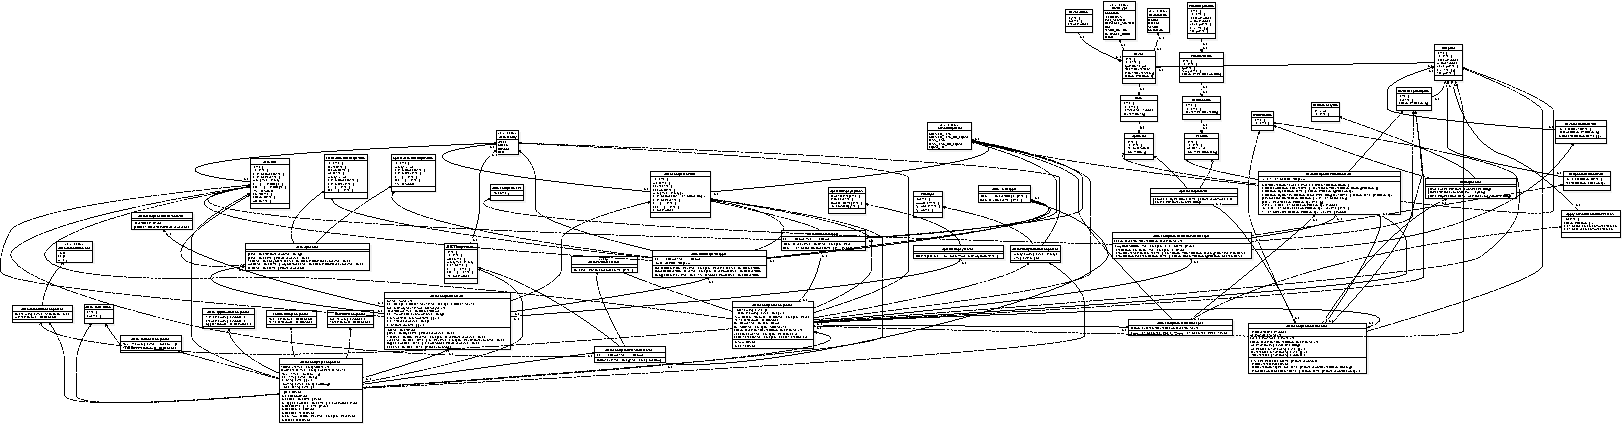
\includegraphics[width=\textwidth]{./frontend/alarm-configuration/alarm-configuration.pdf}
\captionof{figure}{Diagramma delle classi del modulo Alarm-configuration}
\end{center}

\addAtr{+}{mode: InputSignal$<$'create' $|$ 'edit'$>$}{}
\addAtr{+}{initialRule: InputSignal$<$AlarmRule $|$ null$>$}{}
\addAtr{+}{submittedForm: OutputEmitterRef$<$AlarmConfigFormValue$>$}{}
\addAtr{+}{cancelled: OutputEmitterRef$<$void$>$}{}
\addAtr{-}{fb: FormBuilder}{}
\addAtr{-}{formMapper: AlarmRuleFormMapper}{}
\addAtr{-}{formState: AlarmConfigFormStateService}{}
\addAtr{-}{datapointExtraction: DeviceDatapointExtractionService}{}
\addAtr{-}{validationHelper: AlarmConfigFormValidationHelper}{}
\addAtr{-}{fieldOrchestrator: AlarmConfigFormFieldOrchestratorHelper}{}
\addAtr{-}{destroyRef: DestroyRef}{}
\addAtr{-}{editDatapointLookupVersion: number}{}
\addAtr{+}{form: FormGroup}{}
\addAtr{+}{isEditMode: Signal$<$boolean$>$}{}
\addAtr{+}{plants: Signal$<$PlantOption[]$>$}{}
\addAtr{+}{deviceOptions: WritableSignal$<$DeviceDatapointOption[]$>$}{}
\addAtr{+}{datapointOptions: WritableSignal$<$Datapoint[]$>$}{}
\addAtr{+}{plantsLoadError: Signal$<$string $|$ null$>$}{}
\addAtr{+}{devicesLoadError: Signal$<$string $|$ null$>$}{}
\addAtr{+}{isDevicesLoading: Signal$<$boolean$>$}{}
\addAtr{+}{selectedDeviceId: WritableSignal$<$string$>$}{}
\addAtr{+}{selectedDatapointId: WritableSignal$<$string$>$}{}
\addAtr{+}{selectedDatapoint: WritableSignal$<$Datapoint $|$ null$>$}{}
\addAtr{+}{isPlantSelectionVisible: Signal$<$boolean$>$}{}
\addAtr{+}{editPosition: Signal$<$string$>$}{}
\addAtr{+}{priorityOptions: AlarmPriority[]}{}
\addAtr{+}{thresholdOperatorOptions: Signal$<$ThresholdOperator[]$>$}{}
\addAtr{+}{thresholdValueEnumHints: Signal$<$string[]$>$}{}
\addAtr{+}{thresholdValueHelpText: Signal$<$string$>$}{}
\addMet{+}{onSubmit() : void}{Valida il form, normalizza il valore di soglia se necessario ed emette i dati tramite l'evento submittedForm.}
\addMet{+}{onCancel() : void}{Emette l'evento cancelled per segnalare la rinuncia alla compilazione del form.}
\addMet{-}{buildForm() : FormGroup}{Costruisce e restituisce il form reattivo con tutti i campi e i relativi validatori.}
\addMet{-}{createEmptyFormValue() : AlarmConfigFormValue}{Restituisce il valore iniziale vuoto del form da utilizzare in modalità creazione.}
\addMet{-}{applyModeState() : void}{Delega all'orchestratore l'abilitazione o disabilitazione dei campi del form in base alla modalità corrente.}
\addMet{-}{ensurePlantsLoaded() : void}{Delega al servizio di stato il caricamento degli impianti disponibili se non ancora caricati.}
\addMet{-}{onPlantChanged(plantId: string) : void}{Gestisce il cambio di impianto selezionato, resettando le opzioni dispositivo e caricando quelle relative al nuovo impianto.}
\addMet{-}{onDeviceChanged(deviceId: string) : void}{Gestisce il cambio di dispositivo selezionato, aggiornando le opzioni datapoint e resettando i vincoli di soglia.}
\addMet{-}{onDatapointChanged(datapointId: string) : void}{Gestisce il cambio di datapoint selezionato, aggiornando il datapoint corrente e i vincoli di soglia.}
\addMet{-}{applyThresholdConstraints(datapoint: Datapoint $|$ null) : void}{Delega all'helper di validazione l'applicazione dei vincoli sui campi di soglia in base al datapoint selezionato.}
\addMet{-}{loadEditDatapointMetadata(deviceId: string, datapointId: string, \\ lookupVersion: number) : void}{Carica i metadati del datapoint associato alla regola in modalità modifica, aggiornando il datapoint selezionato e i vincoli di soglia.}
\makeCl{AlarmConfigFormComponent}{Componente Angular che gestisce il form reattivo per la creazione e la modifica di una regola di allarme. Coordina la selezione a cascata di impianto, dispositivo e datapoint, delegando la validazione e l'orchestrazione dei campi ai relativi servizi helper.}

\addAtr{-}{stateService: AlarmConfigStateService}{}
\addAtr{-}{tablePresenter: AlarmConfigTablePresenterService}{}
\addAtr{+}{columns: readonly AlarmTableColumn[]}{}
\addAtr{+}{alarms: Signal$<$AlarmRule[]$>$}{}
\addAtr{+}{error: Signal$<$string $|$ null$>$}{}
\addAtr{+}{isModalOpen: WritableSignal$<$boolean$>$}{}
\addAtr{+}{editingRule: WritableSignal$<$AlarmRule $|$ null$>$}{}
\addAtr{+}{pendingDelete: WritableSignal$<$\{id: string, name: string\} $|$ null$>$}{}
\addAtr{+}{pendingToggleRuleId: WritableSignal$<$string $|$ null$>$}{}
\addAtr{+}{rows: Signal$<$AlarmConfigTableRow[]$>$}{}
\addAtr{+}{modalTitle: Signal$<$string$>$}{}
\addMet{+}{ngOnInit() : void}{Avvia il caricamento delle regole di allarme tramite il servizio di stato.}
\addMet{+}{onCreateNew() : void}{Reimposta la regola in modifica e apre il modal per la creazione di una nuova regola.}
\addMet{+}{onEdit(alarmRuleId: string) : void}{Recupera la regola corrispondente all'identificativo specificato e apre il modal in modalità modifica.}
\addMet{+}{onToggleEnabled(alarmRuleId: string, enabled: boolean) : void}{Attiva o disattiva la regola specificata tramite il servizio di stato, prevenendo richieste concorrenti.}
\addMet{+}{onDelete(id: string, name: string) : void}{Imposta la regola candidata all'eliminazione per la richiesta di conferma.}
\addMet{+}{onDeleteConfirmed() : void}{Conferma l'eliminazione della regola in attesa e reimposta il segnale pendingDelete.}
\addMet{+}{onDeleteCancelled() : void}{Annulla l'eliminazione in corso reimpostando il segnale pendingDelete a null.}
\addMet{+}{getDeleteConfirmMessage() : string}{Restituisce il messaggio di conferma per l'eliminazione della regola in attesa.}
\addMet{+}{onFormSubmitted(formValue: AlarmConfigFormValue) : void}{Crea o aggiorna la regola di allarme in base alla modalità corrente del form, chiudendo il modal al termine.}
\addMet{+}{onModalClosed() : void}{Chiude il modal e reimposta la regola in modifica a null.}
\makeCl{AlarmConfigPageComponent}{Componente Angular che rappresenta la pagina di configurazione delle regole di allarme, con supporto alla creazione, modifica, eliminazione e attivazione delle regole. Coordina l'apertura del modal di form e i dialog di conferma tramite segnali reattivi.}

\addAtr{-}{datapointExtraction: DeviceDatapointExtractionService}{}
\addMet{+}{applyModeState(form: AlarmConfigFormLike, mode: 'create' $|$ 'edit') : void}{Abilita o disabilita i campi del form e aggiorna i validatori in base alla modalità corrente.}
\addMet{+}{resetDatapointControl(form: AlarmConfigFormLike) : void}{Reimposta il controllo datapointId a stringa vuota e ne aggiorna la validità.}
\addMet{+}{resolveDeviceSelection(deviceId: string, deviceOptions: readonly \\ DeviceDatapointOption[]) : DeviceSelectionResult}{Risolve la selezione del dispositivo restituendo i datapoint leggibili e l'eventuale datapoint auto-selezionato se unico.}
\addMet{+}{resolveDatapointSelection(datapointId: string, datapointOptions: readonly Datapoint[]) : DatapointSelectionResult}{Risolve la selezione del datapoint restituendo l'identificativo normalizzato e il datapoint corrispondente se trovato.}
\makeCl{AlarmConfigFormFieldOrchestratorHelper}{Helper Angular per l'orchestrazione dei campi del form di configurazione allarme. Gestisce l'abilitazione e la validazione dei controlli in base alla modalità e risolve le selezioni a cascata di dispositivo e datapoint.}

\addAtr{-}{datapointExtraction: DeviceDatapointExtractionService}{}
\addMet{+}{applyThresholdConstraints(\{mode, datapoint, \\ thresholdOperatorControl, thresholdValueControl\}: \\ ApplyThresholdConstraintsParams) : void}{Applica i validatori ai controlli di operatore e valore di soglia in base alla modalità e al datapoint selezionato, resettando l'operatore se non più consentito.}
\addMet{-}{resolveAllowedOperators(mode: 'create' $|$ 'edit', datapoint: Datapoint $|$ null, \\ currentOperator: ThresholdOperator $|$ null) : \\ ThresholdOperator[]}{Restituisce la lista degli operatori consentiti in base al datapoint selezionato e alla modalità corrente.}
\addMet{-}{operatorAllowedValidator(allowedOperators: readonly ThresholdOperator[]) : ValidatorFn}{Restituisce un validatore che verifica se l'operatore selezionato è tra quelli consentiti.}
\addMet{-}{enumThresholdValidator(enumValues: readonly string[]) : ValidatorFn}{Restituisce un validatore che verifica se il valore di soglia inserito appartiene ai valori enumerati previsti dal datapoint.}
\makeCl{AlarmConfigFormValidationHelper}{Helper Angular per la gestione della validazione dei campi di soglia nel form di configurazione allarme. Applica dinamicamente i validatori appropriati in base al datapoint selezionato e alla modalità del form.}

\addAtr{-}{alarmTimeMapper: AlarmTimeMapper}{}
\addMet{+}{toFormValue(rule: AlarmRule) : AlarmConfigFormValue}{Trasforma una regola di allarme nel corrispondente valore del form di configurazione.}
\addMet{-}{toFormThresholdOperator(operator: string) : ThresholdOperator}{Converte una stringa rappresentante un operatore di soglia nell'enumerato ThresholdOperator corrispondente, lanciando un errore se non riconosciuto.}
\makeCl{AlarmRuleFormMapper}{Mapper Angular per la trasformazione di una regola di allarme nel formato atteso dal form di configurazione. Delega la conversione degli orari all'AlarmTimeMapper e gestisce la mappatura degli operatori di soglia.}

\addAtr{-}{alarmTimeMapper: AlarmTimeMapper}{}
\addAtr{-}{hourMinutePattern: RegExp}{}
\addMet{+}{toCreateRequest(formValue: AlarmConfigFormValue) : CreateAlarmRuleRequestDto}{Trasforma il valore del form nel DTO di richiesta per la creazione di una nuova regola di allarme.}
\addMet{+}{toUpdateRequest(formValue: AlarmConfigFormValue) : UpdateAlarmRuleRequestDto}{Trasforma il valore del form nel DTO di richiesta per l'aggiornamento di una regola di allarme esistente.}
\addMet{+}{toToggleRequest(rule: AlarmRule, isArmed: boolean) : UpdateAlarmRuleRequestDto}{Costruisce il DTO di aggiornamento per la sola modifica dello stato di armamento di una regola esistente.}
\addMet{-}{toPriorityNumber(priority: AlarmPriority $|$ null) : number}{Estrae il valore numerico della priorità, lanciando un errore se null.}
\addMet{-}{toThresholdOperatorCode(operator: ThresholdOperator $|$ null) : string}{Converte l'enumerato ThresholdOperator nel codice stringa corrispondente, lanciando un errore se non riconosciuto.}
\addMet{-}{requireField$<$T$>$(value: T $|$ null, fieldName: string) : T}{Verifica che il valore non sia null, lanciando un errore con il nome del campo se mancante.}
\addMet{-}{requireNonEmptyString(value: string, fieldName: string) : string}{Verifica che la stringa non sia vuota dopo il trim, lanciando un errore con il nome del campo se vuota.}
\addMet{-}{normalizeOptionalString(value?: string) : string $|$ undefined}{Normalizza una stringa opzionale restituendo undefined se vuota dopo il trim.}
\addMet{-}{requireHourMinuteString(value: string, fieldName: string) : string}{Verifica che la stringa rispetti il formato HH:MM, lanciando un errore se non conforme.}
\addMet{-}{requireThresholdOperator(operator: string) : string}{Verifica che la stringa sia un operatore di soglia valido, lanciando un errore altrimenti.}
\addMet{-}{toRequestThresholdValue(value: string, fieldName: string) : string}{Normalizza il valore di soglia convertendo le varianti booleane nei valori canonici on/off.}
\makeCl{AlarmRuleRequestMapper}{Mapper Angular per la costruzione dei DTO di creazione, aggiornamento e toggle delle regole di allarme a partire dai valori del form o da una regola esistente. Gestisce la validazione e la normalizzazione di tutti i campi obbligatori prima della serializzazione.}

\addMet{+}{toFormTime(value: Date $|$ string) : string}{Converte un valore di tipo Date o stringa nel formato orario HH:MM utilizzato dal form, gestendo i formati ISO, HH:MM e HH:MM:SS.}
\addMet{-}{toHourMinute(value: string) : string}{Estrae i componenti ora e minuto da una stringa in formato ISO o la tronca ai primi cinque caratteri se il pattern non corrisponde.}
\makeCl{AlarmTimeMapper}{Mapper Angular per la conversione di valori temporali nel formato HH:MM richiesto dal form di configurazione allarme. Gestisce diversi formati di input tra cui Date, ISO 8601, HH:MM e HH:MM:SS.}

\addAtr{+}{name: string}{}
\addAtr{+}{plantId: string}{}
\addAtr{+}{deviceId: string}{}
\addAtr{+}{datapointId?: string}{}
\addAtr{+}{priority: AlarmPriority $|$ null}{}
\addAtr{+}{thresholdOperator: ThresholdOperator $|$ null}{}
\addAtr{+}{thresholdValue: string}{}
\addAtr{+}{armingTime: string}{}
\addAtr{+}{dearmingTime: string}{}
\addAtr{+}{enabled: boolean}{}
\makeAbCl{AlarmConfigFormValue}{Interfaccia che rappresenta il valore del form di configurazione di una regola di allarme. Raccoglie tutti i campi necessari per la creazione e la modifica di una regola, inclusi dispositivo, datapoint, soglia e orari di armamento.}

\addAtr{+}{id: string}{}
\addAtr{+}{name: string}{}
\addAtr{+}{position: string}{}
\addAtr{+}{priority: AlarmPriority}{}
\addAtr{+}{threshold: string}{}
\addAtr{+}{armingTime: string}{}
\addAtr{+}{dearmingTime: string}{}
\addAtr{+}{isEnabled: boolean}{}
\makeAbCl{AlarmConfigTableRow}{Tipo che rappresenta una riga della tabella di configurazione delle regole di allarme. Raccoglie le informazioni di posizione, priorità, soglia e orari di armamento da visualizzare nella tabella.}

\addAtr{-}{hasRequestedPlants: boolean}{}
\addAtr{-}{wardApi: WardApiService}{}
\addAtr{-}{apartmentApi: ApartmentApiService}{}
\addAtr{-}{datapointExtraction: DeviceDatapointExtractionService}{}
\addAtr{+}{plants: WritableSignal$<$WardPlantDto[]$>$}{}
\addAtr{+}{plantsLoadError: WritableSignal$<$string $|$ null$>$}{}
\addAtr{+}{devicesLoadError: WritableSignal$<$string $|$ null$>$}{}
\addAtr{+}{isDevicesLoading: WritableSignal$<$boolean$>$}{}
\addMet{+}{ensurePlantsLoaded(mode: 'create' $|$ 'edit') : Observable$<$void$>$}{Carica la lista degli impianti disponibili se non ancora caricata e la modalità è di creazione, aggiornando il segnale plants o l'errore in caso di fallimento.}
\addMet{+}{resetDevicesLoadState() : void}{Reimposta l'errore di caricamento dispositivi e il flag di caricamento in corso.}
\addMet{+}{loadDeviceOptionsByPlant(plantId: string) : Observable$<$DeviceDatapointOption[]$>$}{Carica le opzioni dispositivo per l'impianto specificato, aggiornando lo stato di caricamento e restituendo un array vuoto in caso di errore.}
\addMet{+}{resolveDatapointForEdit(deviceId: string, datapointId: string) : \\ Observable$<$Datapoint $|$ null$>$}{Ricerca il datapoint corrispondente agli identificativi forniti tra tutti gli impianti disponibili, restituendo null se non trovato o in caso di errore.}
\addMet{-}{loadAllPlants() : Observable$<$WardPlantDto[]$>$}{Recupera tutti gli impianti disponibili combinando quelli dei ward e quelli generici, deduplicando e ordinando il risultato per nome.}
\addMet{-}{mergePlants(availablePlants: WardPlantDto[], \\ assignedPlants: WardPlantDto[]) : WardPlantDto[]}{Unisce due liste di impianti deduplicando per identificativo e ordinando il risultato alfabeticamente per nome.}
\makeCl{AlarmConfigFormStateService}{Servizio Angular per la gestione dello stato del form di configurazione allarme, con scope a livello di componente. Gestisce il caricamento degli impianti e delle opzioni dispositivo, esponendo segnali reattivi per lo stato di caricamento e gli eventuali errori.}

\addAtr{-}{api: AlarmApiService}{}
\addAtr{-}{alarmManagementRefreshService: AlarmManagementRefreshService}{}
\addAtr{-}{apiErrorDisplayService: ApiErrorDisplayService}{}
\addAtr{-}{requestMapper: AlarmRuleRequestMapper}{}
\addAtr{-}{alarmsSubject: BehaviorSubject$<$AlarmRule[]$>$}{}
\addAtr{-}{errorSubject: BehaviorSubject$<$string $|$ null$>$}{}
\addAtr{+}{alarms\$: Observable$<$AlarmRule[]$>$}{}
\addAtr{+}{error\$: Observable$<$string $|$ null$>$}{}
\addMet{+}{loadAlarmRules() : void}{Carica la lista delle regole di allarme dal backend e aggiorna il subject interno, impostando l'errore in caso di fallimento.}
\addMet{+}{getAlarmRuleById(id: string) : Observable$<$AlarmRule$>$}{Recupera la singola regola di allarme corrispondente all'identificativo specificato.}
\addMet{+}{createAlarmRule(formValue: AlarmConfigFormValue) : Observable$<$AlarmRule$>$}{Mappa il valore del form nel DTO di creazione e invia la richiesta al backend, ricaricando la lista al termine.}
\addMet{+}{updateAlarmRule(alarmId: string, formValue: AlarmConfigFormValue) : \\ Observable$<$AlarmRule$>$}{Mappa il valore del form nel DTO di aggiornamento e invia la richiesta al backend, ricaricando la lista al termine.}
\addMet{+}{toggleEnabled(alarmId: string, enabled: boolean) : Observable$<$AlarmRule$>$}{Aggiorna lo stato di armamento della regola specificata, costruendo il DTO a partire dallo stato locale corrente.}
\addMet{+}{deleteAlarmRule(alarmId: string) : Observable$<$void$>$}{Elimina la regola di allarme specificata e aggiorna la lista locale rimuovendo l'elemento eliminato.}
\addMet{-}{clearError() : void}{Reimposta il subject degli errori a null se contiene un valore.}
\addMet{-}{handleError$<$T$>$(message: string) : Observable$<$T$>$}{Imposta il messaggio di errore nel subject e restituisce EMPTY per interrompere il flusso.}
\addMet{-}{handleApiError$<$T$>$(fallbackMessage: string) : OperatorFunction$<$T, T$>$}{Restituisce un operatore RxJS che intercetta gli errori API, formattando il messaggio tramite il servizio di display degli errori.}
\addMet{-}{reloadAlarmsAfterMutation() : void}{Ricarica la lista delle regole di allarme e notifica il servizio di refresh dopo una mutazione.}
\makeCl{AlarmConfigStateService}{Servizio Angular con scope a livello di componente per la gestione dello stato delle regole di allarme nella pagina di configurazione. Coordina le operazioni CRUD delegando le chiamate API al servizio dedicato e mantenendo la lista aggiornata tramite BehaviorSubject.}

\addAtr{-}{alarmTimeMapper: AlarmTimeMapper}{}
\addMet{+}{toRows(rules: AlarmRule[]) : AlarmConfigTableRow[]}{Trasforma una lista di regole di allarme nelle corrispondenti righe della tabella di configurazione, formattando posizione, soglia e orari.}
\makeCl{AlarmConfigTablePresenterService}{Servizio Angular per la trasformazione delle regole di allarme nel formato di presentazione della tabella di configurazione. Delega la conversione degli orari all'AlarmTimeMapper e formatta la soglia combinando operatore e valore.}

\addAtr{-}{numericThresholdPattern: RegExp}{}
\addMet{+}{extractDeviceOptions(apartment: Apartment) : DeviceDatapointOption[]}{Estrae le opzioni dispositivo da un appartamento, costruendo l'etichetta combinando nome stanza e nome dispositivo.}
\addMet{+}{findReadableDatapoints(deviceId: string, deviceOptions: \\ readonly DeviceDatapointOption[]) : Datapoint[]}{Restituisce i datapoint leggibili del dispositivo corrispondente all'identificativo specificato.}
\addMet{+}{findDatapointById(datapointId: string, \\ datapoints: readonly Datapoint[]) : Datapoint $|$ null}{Cerca e restituisce il datapoint corrispondente all'identificativo specificato, o null se non trovato.}
\addMet{+}{findDatapointByDeviceAndDatapointId(plants: readonly PlantDto[], deviceId: string, datapointId: string) : Datapoint $|$ null}{Ricerca il datapoint corrispondente agli identificativi di dispositivo e datapoint tra tutti gli impianti forniti.}
\addMet{+}{getAllowedOperators(datapoint: Datapoint $|$ null) : ThresholdOperator[]}{Restituisce gli operatori di soglia consentiti per il datapoint specificato, limitando a EQUAL\_TO per i datapoint enumerati.}
\addMet{+}{getEnumValues(datapoint: Datapoint $|$ null) : string[]}{Restituisce i valori enumerati normalizzati del datapoint specificato, o un array vuoto se assente.}
\addMet{+}{usesEnumeratedThreshold(datapoint: Datapoint $|$ null) : boolean}{Verifica se il datapoint richiede una soglia enumerata anziché numerica.}
\addMet{+}{normalizeThresholdValue(datapoint: Datapoint $|$ null, value: string) : string}{Normalizza il valore di soglia cercando una corrispondenza case-insensitive tra i valori enumerati del datapoint.}
\addMet{+}{isThresholdValueValid(datapoint: Datapoint $|$ null, value: string) : boolean}{Verifica se il valore di soglia è valido rispetto ai valori enumerati o al pattern numerico del datapoint.}
\addMet{-}{normalizeDatapoints(datapoints: readonly Datapoint[] $|$ undefined) : Datapoint[]}{Normalizza la lista di datapoint applicando la normalizzazione dei valori enumerati a ciascuno.}
\addMet{-}{normalizeEnumValues(values: readonly string[] $|$ undefined) : string[]}{Normalizza i valori enumerati rimuovendo spazi, filtrando i vuoti e deduplicando.}
\makeCl{DeviceDatapointExtractionService}{Servizio Angular per l'estrazione e la normalizzazione dei datapoint dei dispositivi, con supporto alla ricerca per identificativo e alla validazione dei valori di soglia. Determina gli operatori consentiti e il tipo di soglia in base alle caratteristiche del datapoint selezionato.}